%=================================================================

\section{Introduction}\label{sec-intro}


%\todo{Narrow down to a topic; Dig a hole; Fill the hole}




%\gangli{``narrow in on topic'' reminds you 
%that readers and reviewers only know that this is a AI or HTM research paper (and maybe have read the title/abstract). 
%You need to help them figure out what topic and area of research paper this is. 
%You _don't_ need to wax poetic about the topic's importance.}

%\gangli{`dig a hole'' reminds you that 
%you need to convince the reader that there's a problem with the state of the world. 
%Prior work may exist but it's either missing something important or there's a missing opportunity. 
%The reader should be drooling for a bright future just out of reach.}

%\gangli{``fill the hole'' reminds you to show the reader 
%how and why the paper they're reading will fix these problems and deliver us into a better place. 
%You don't need a whirlwind summary of the technical details, 
%but you need readers convinced (and in a good mood) to keep reading.}





%\todo{The importance of the area}
%\blindtext

Sales forecasting using time series is one of the most important applications in business and economics. It helps businesses make production plans, inventory management, sales and marketing strategies, etc. based on the predicted future sales. Time series forecasting can be done using various models and algorithms such as linear regression, exponential smoothing, ARIMA, neural networks, etc. 


%\todo{The problems faced by most current methods}
%\blindtext

This sales forecasting task has multiple factors that need to be considered. It is necessary to take into account the impact of multiple factors on the forecasting goal.Consider how to perform data analysis to simplify the model prediction goal.

%\todo{What can be addressed by existing methods; Why those problems are challenges to existing methods?}
%\blindtext







\section{Data Analysis} \label{sec-preliminaries}
The data covers six countries: Belgium, France, Germany, Italy, Poland, Spain, two stores: KaggleMart, KaggleRama, and four products.The training set timeline is from 2017 to 2020, and the test set timeline is 2021.
Firstly, the monthly sales volume of the overall data is analyzed. This paper finds that there is a cyclical trend in the change of sales.

\begin{figure}[!h]
		\centering
		\selectcolormodel{rgb}
		\includegraphics[scale=0.23]{month.eps}
		%  \includegraphics[width=0.5\textwidth]{figures//OutAspect_target.eps}\\
		\caption{Monthly sales}\label{fig:OutAspect-target}
\end{figure}
Analysis of the store factors will be conducted next. By calculating the daily sales ratio of each store, it is found that KaggleMart's sales ratio remains around 75\%, while KaggleRama's sales ratio is 25\%. This indicates that the sales ratio of stores is almost fixed and unchanged.



\begin{figure}[H]
	\centering
	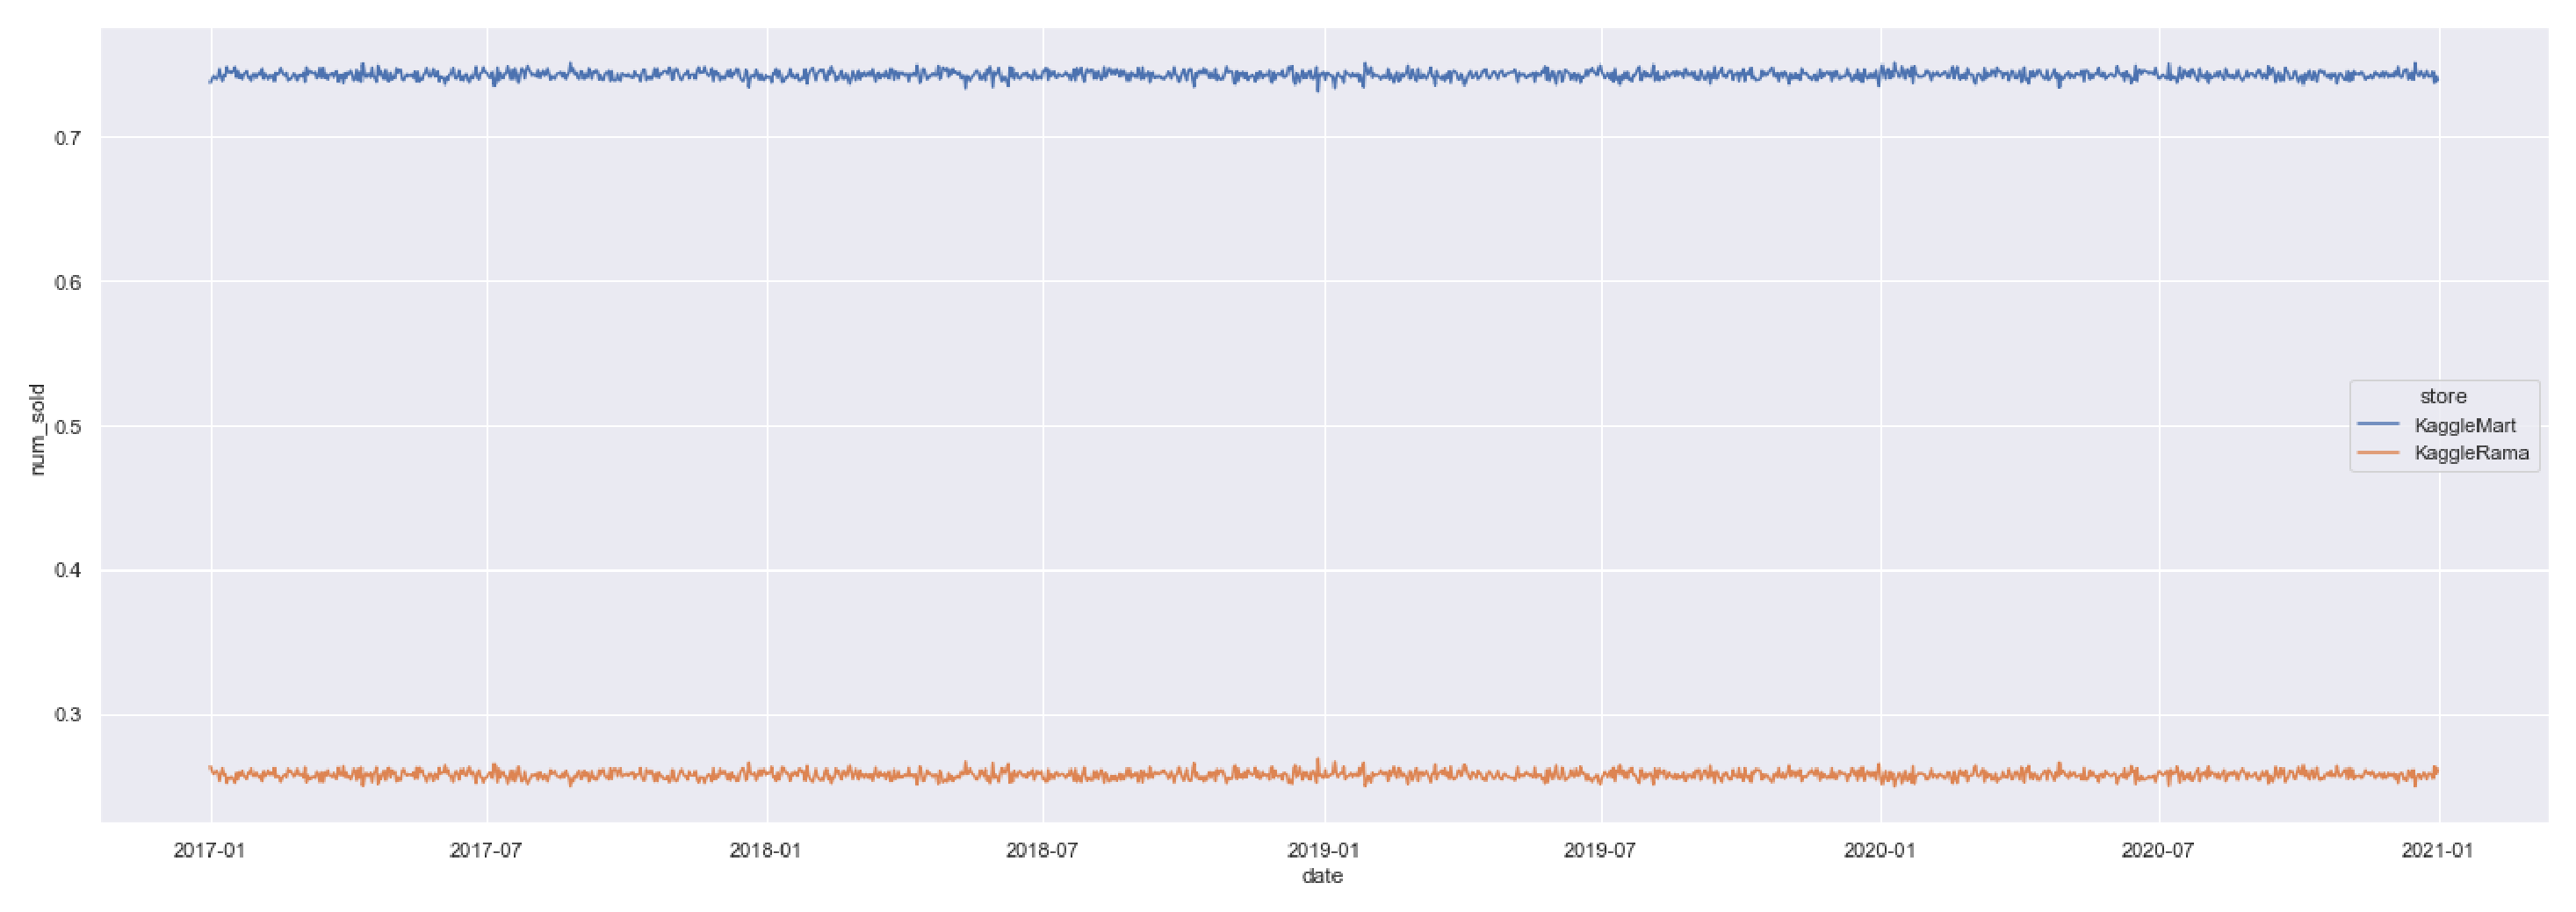
\includegraphics[scale=0.21]{store-ratio.eps}
	%  \includegraphics[width=0.5\textwidth]{figures//OutAspect_target.eps}\\
	\caption{Stores ratio}\label{fig:OutAspect-target}
\end{figure}

For more intuitive performance, this paper takes the sales volume of KaggleMart as the benchmark, and multiplies the sales volume of KaggleRama by a weight value to remove the impact of the ratio. The observation chart shows that their sales volume change curves almost coincide, indicating that their sales volume is only related to the total sales volume and has nothing to do with the factors of the store itself.

\begin{figure}[htb]
	\centering
	\selectcolormodel{rgb}
	\includegraphics[scale=0.225]{store-trend.eps}
	%  \includegraphics[width=0.5\textwidth]{figures//OutAspect_target.eps}\\
	\caption{Stores ratio trend}\label{fig:OutAspect-target}
\end{figure}
We analyzed the national factors in the same way and found similar phenomena. The sales volume of each country is different before 2020, and the proportion is almost fixed, while the proportion of six countries is the same in 2020. It can also exclude the influence of the country itself and predict the sales volume of each country through the total sales volume.

\begin{figure}[h]
	\centering
	\selectcolormodel{rgb}
	\includegraphics[scale=0.215]{Country-ratio.eps}
	%  \includegraphics[width=0.5\textwidth]{figures//OutAspect_target.eps}\\
	\caption{Countries ratio}\label{fig:OutAspect-target}
\end{figure}
\begin{figure}[h]
	\centering
	\selectcolormodel{rgb}
	\includegraphics[scale=0.235]{Country-trend.eps}
	%  \includegraphics[width=0.5\textwidth]{figures//OutAspect_target.eps}\\
	\caption{Countries ratio trend}\label{fig:OutAspect-target}
\end{figure}

Finally, we will analyze the store and the country together, and use the KaggleMart of Belgium as the benchmark to draw the broken line chart of the flower removal rate. It was found that the sales curve almost coincided.

		\begin{figure}[H]
	\centering
	\selectcolormodel{rgb}
	\includegraphics[scale=0.23]{Countryandstore-trend.eps}
	%  \includegraphics[width=0.5\textwidth]{figures//OutAspect_target.eps}\\
	\caption{Countries and Store trend}\label{fig:OutAspect-target}
	\end{figure}

After that, we analyzed the change of the proportion of the four commodities and found that there was a two-year cycle of change.

		\begin{figure}[H]
	\centering
	\selectcolormodel{rgb}
	\includegraphics[scale=0.3]{product-trend.eps}
	%  \includegraphics[width=0.5\textwidth]{figures//OutAspect_target.eps}\\
	\caption{Product ratio trend}\label{fig:OutAspect-target}
\end{figure}

Therefore, we can only predict the total sales volume of each day by aggregating the time series, and then predict the sales volume of various products in stores in various countries by the total sales volume.

\begin{figure}[h]
	\centering
	\selectcolormodel{rgb}
	\includegraphics[scale=0.3]{trainline.eps}
	%  \includegraphics[width=0.5\textwidth]{figures//OutAspect_target.eps}\\
	\caption{Aggregated time series}\label{fig:OutAspect-target}
\end{figure}

\section{Feature Extraction} \label{sec-method}

Through the above data analysis, we found that we can predict all results as long as we predict the total daily sales and the proportion of product sales. Therefore, we need to extract the time feature of the training set.

By analyzing the sales curve of a week, we find that the sales volume from Sunday to Wednesday is almost the same, while the sales volume from Thursday to Saturday is different every day, so we can extract the time feature of a week.

	\begin{figure}[H]
	\centering
	\selectcolormodel{rgb}
	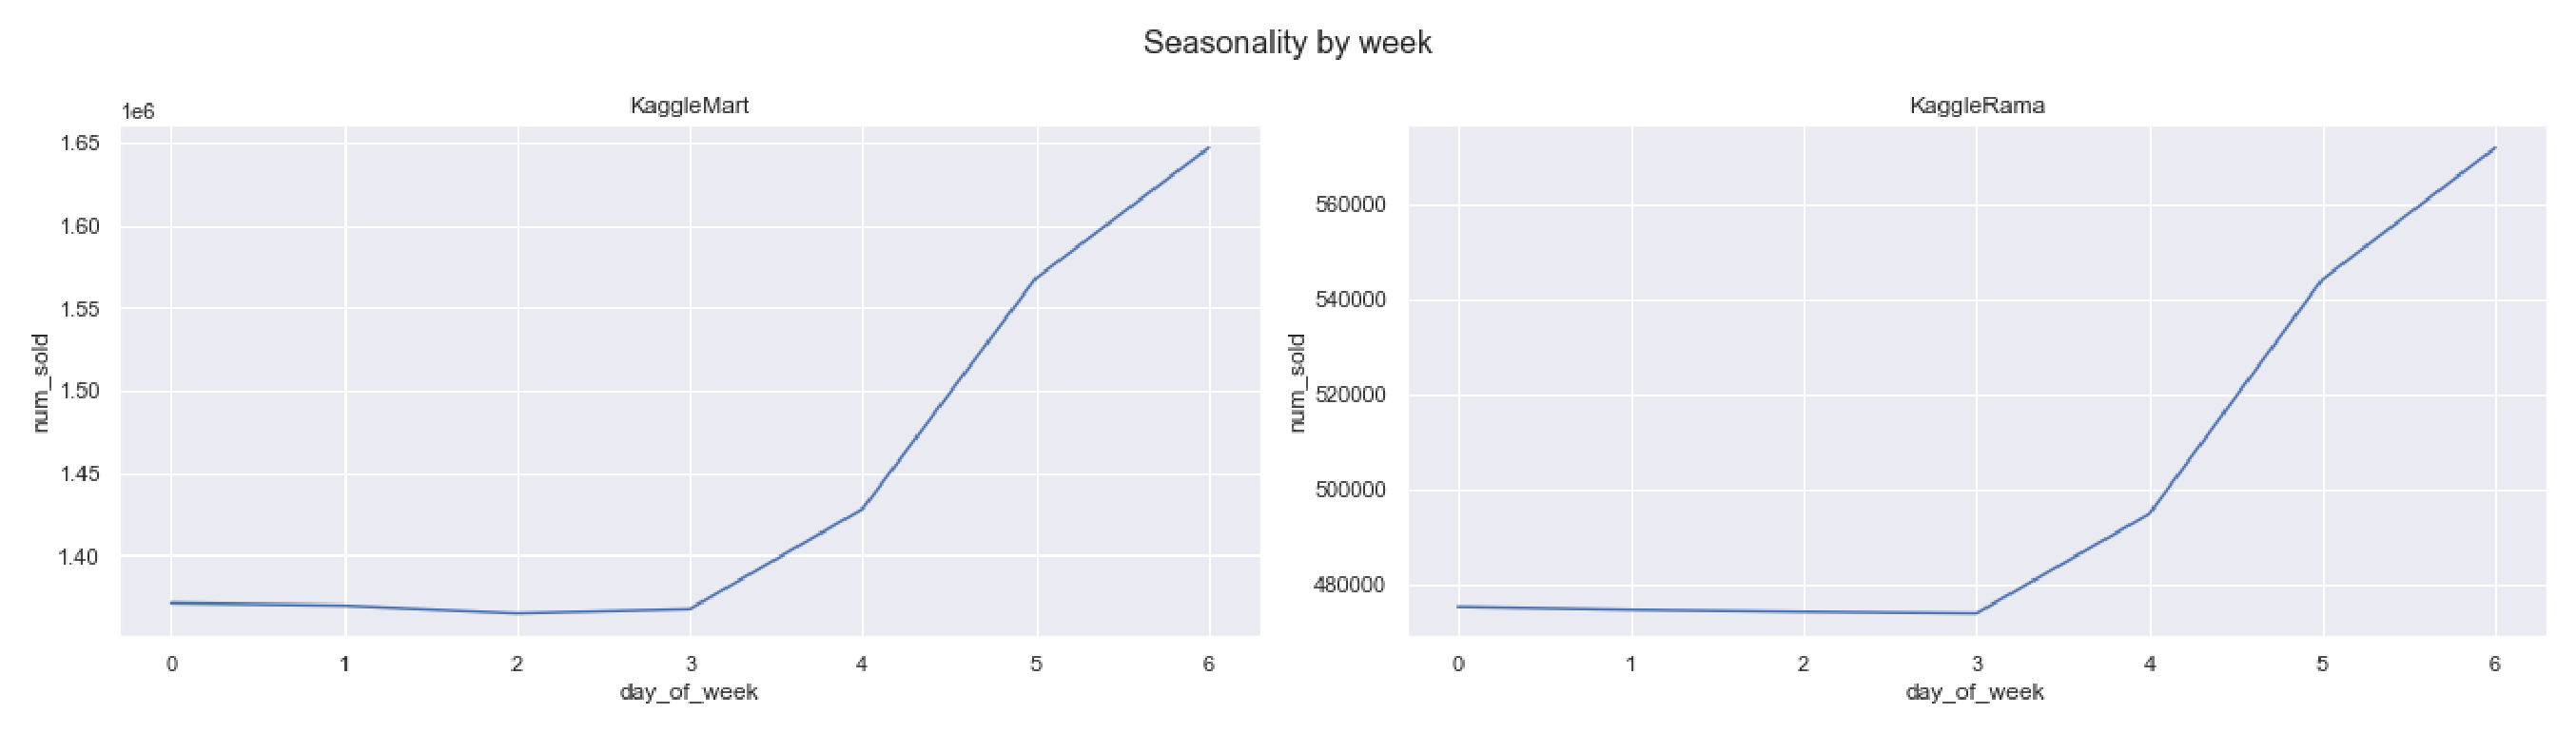
\includegraphics[scale=0.25]{week-feature.eps}
	%  \includegraphics[width=0.5\textwidth]{figures//OutAspect_target.eps}\\
	\caption{weekday feature}\label{fig:OutAspect-target}
\end{figure}
At the same time, in order to make Fourier transform understand the monthly data, we remove the sine value and cosine value of the month. At the same time, we also considered the feature of important festivals in the year. Finally, we get that the features of the training set include 23 features.

\section{Model Train} \label{sec-experiment}
We use Ridge regression from the "linear_model" module to correlate the relationship betweensales and time features , and predict on the test set.Train the model with time features as X and sales as y.The sales of the test set is predicted according to the time features of the test set.Finally, we obtained the total sales prediction curve.

\begin{figure}[H]
	\centering
	\selectcolormodel{rgb}
	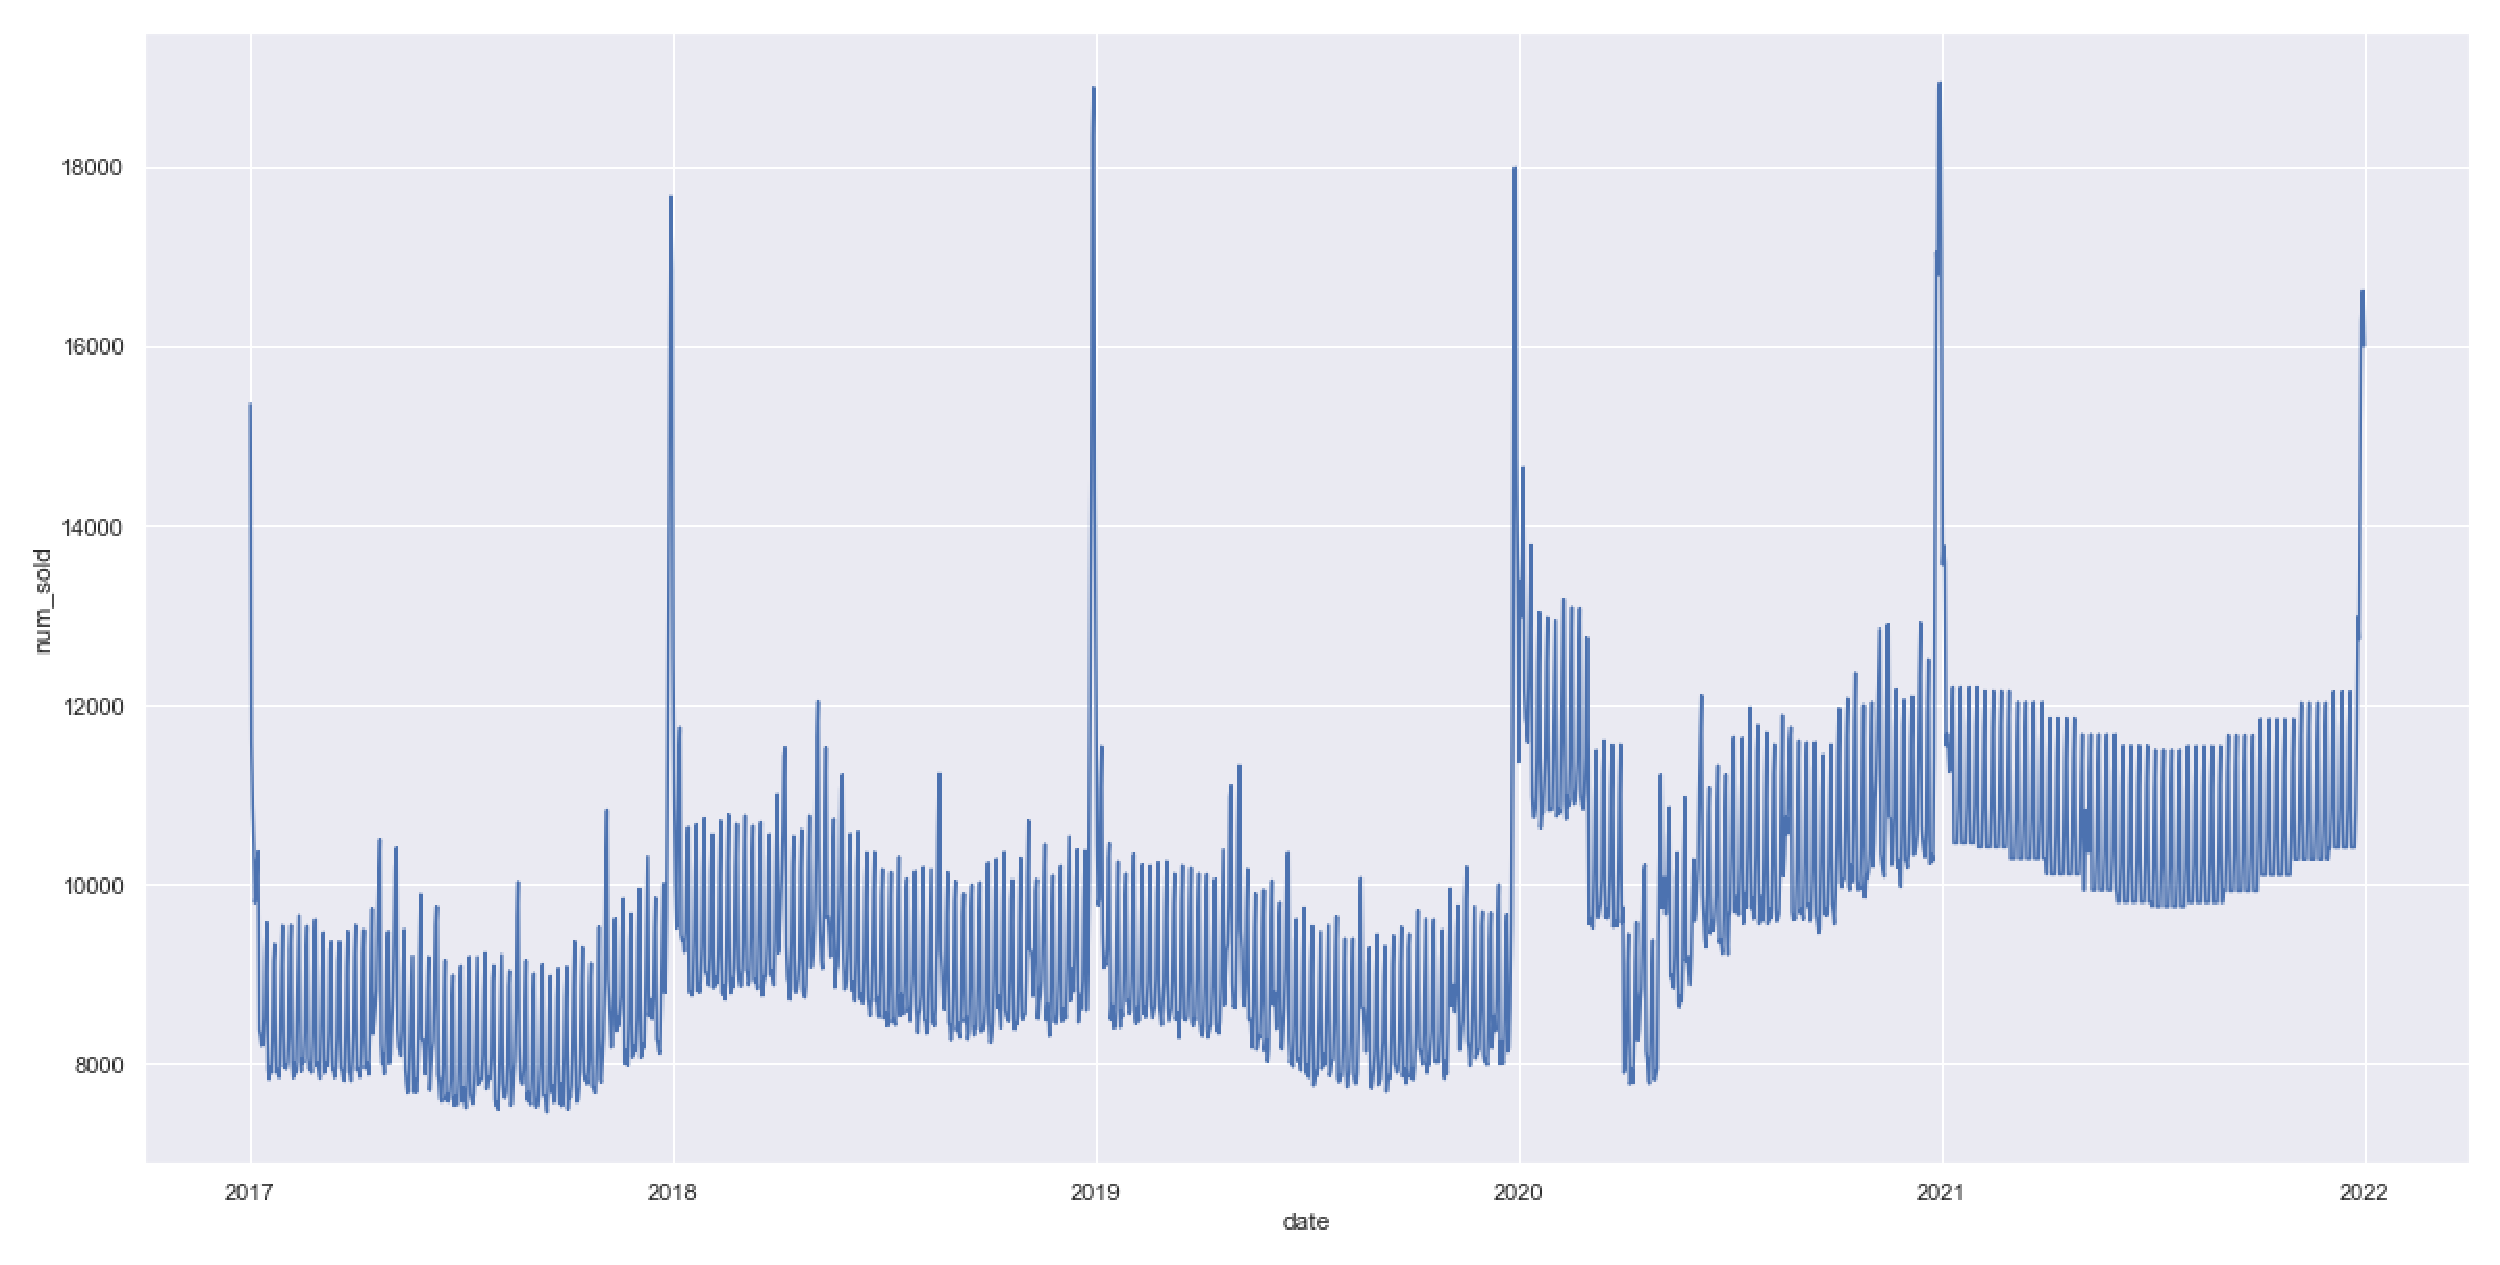
\includegraphics[scale=0.3]{total-sales.eps}
	%  \includegraphics[width=0.5\textwidth]{figures//OutAspect_target.eps}\\
	\caption{total sales forecasting}\label{fig:OutAspect-target}
\end{figure}

We found that the proportion of sales for a product has a cyclical variation with a period of two years. Therefore, we assign the daily proportion of sales for each product in 2019 to 2021.

	\begin{figure}[htb]
	\centering
	\selectcolormodel{rgb}
	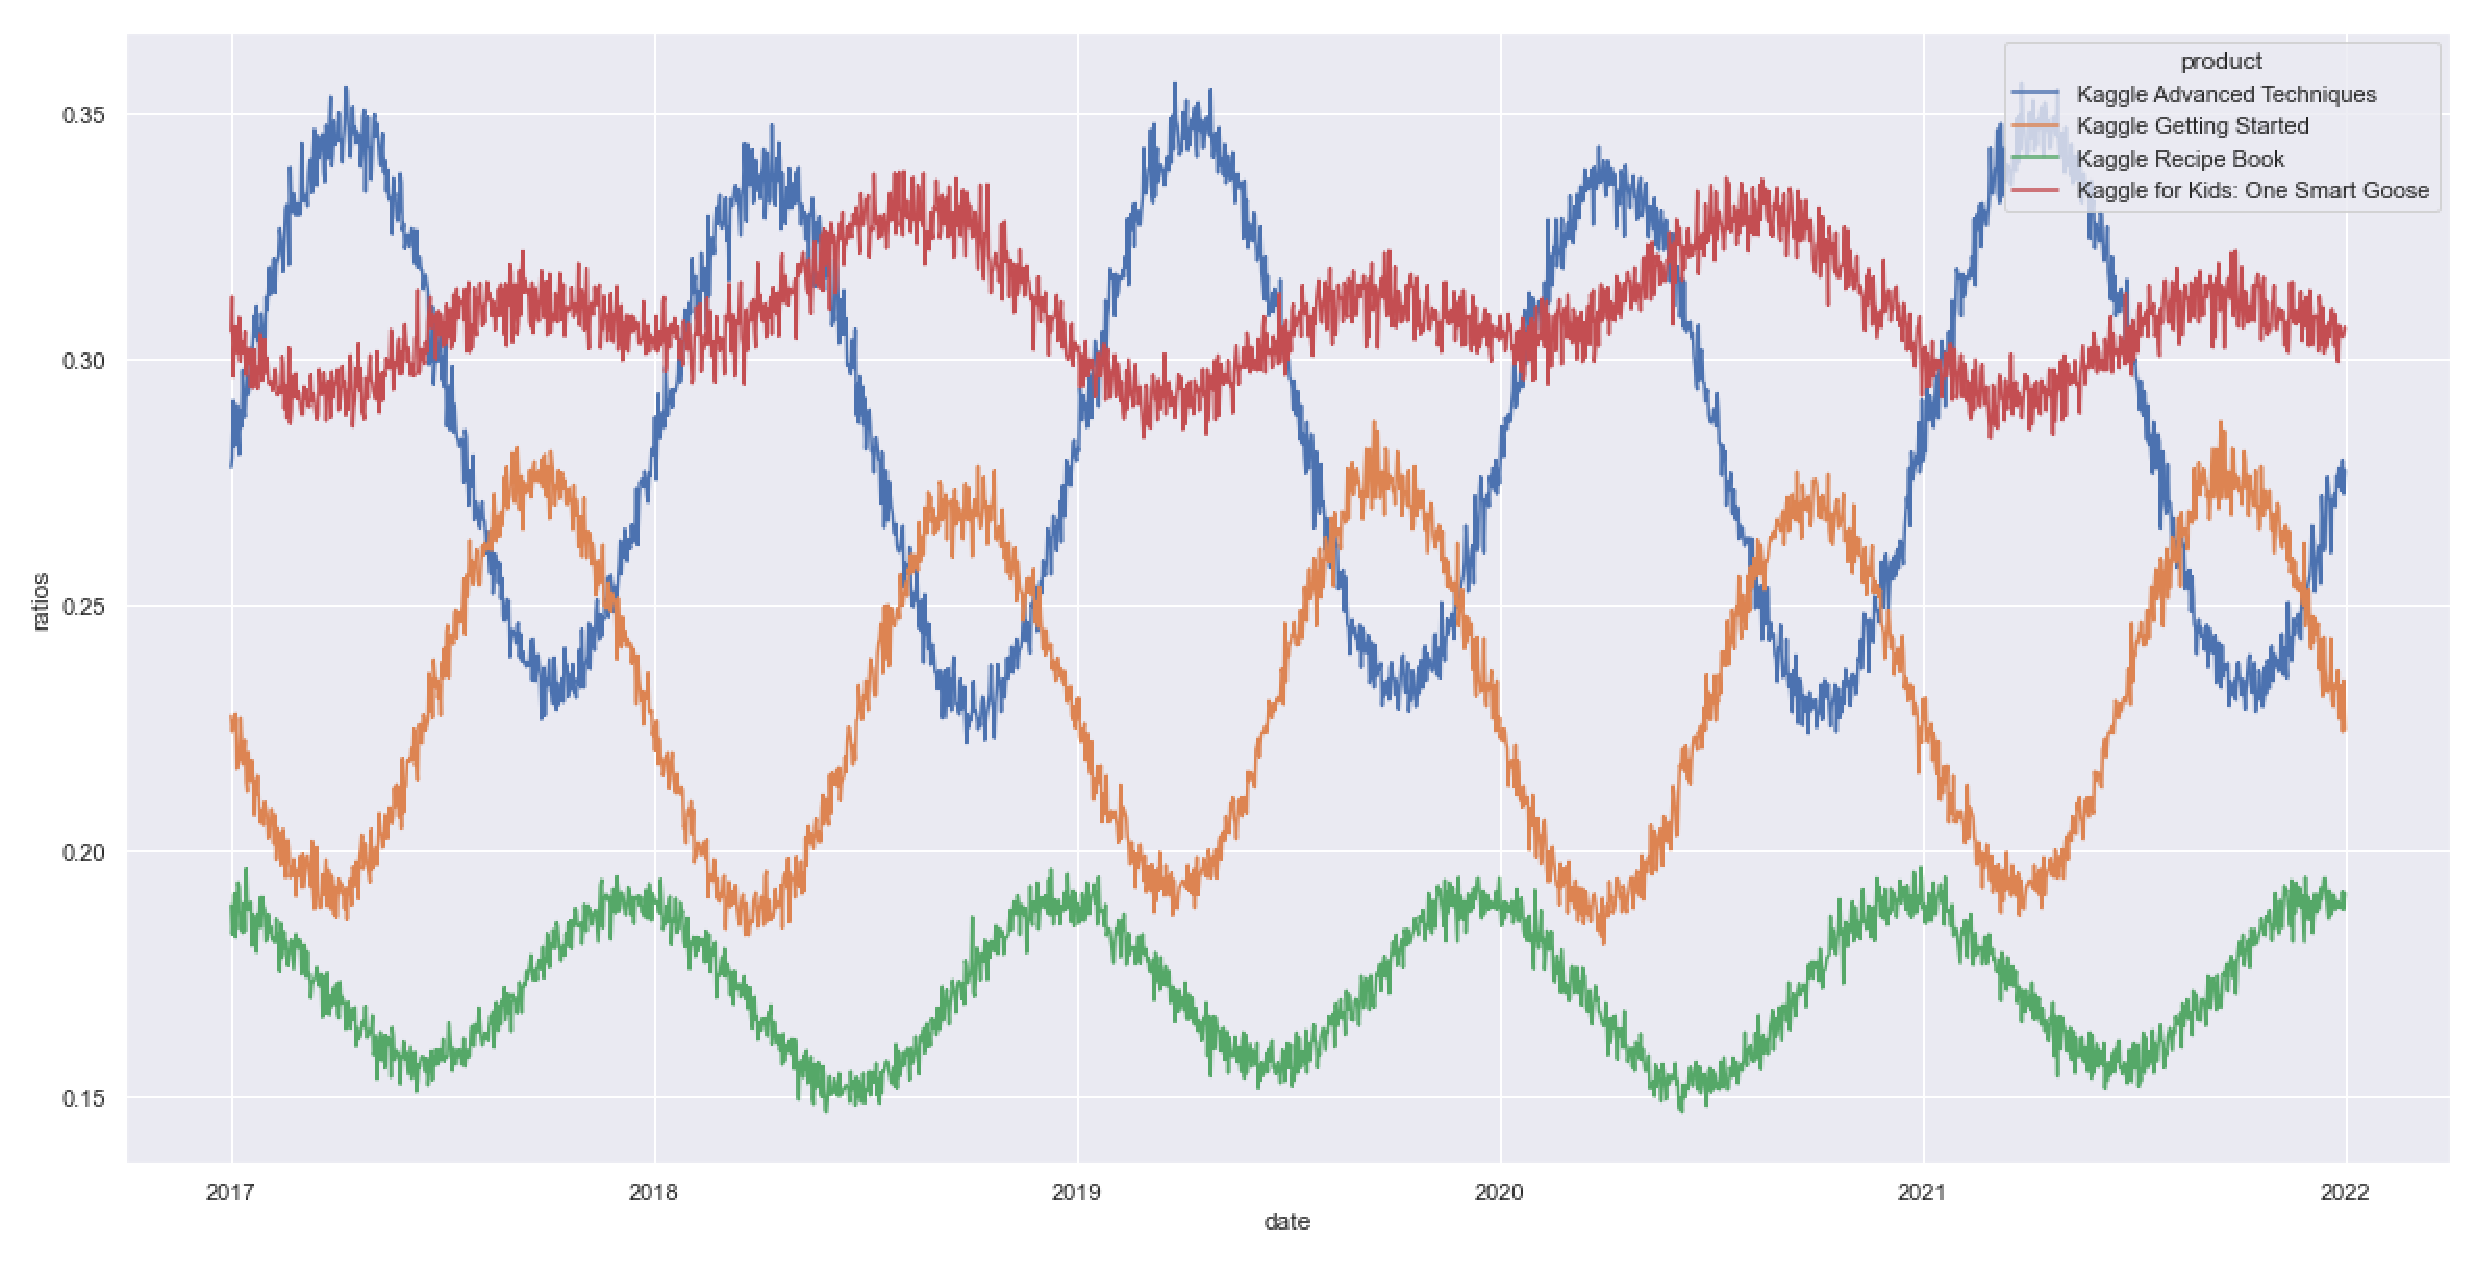
\includegraphics[scale=0.3]{product-ratio-for.eps}
	%  \includegraphics[width=0.5\textwidth]{figures//OutAspect_target.eps}\\
	\caption{Product Ratio Forecast}\label{fig:OutAspect-target}
\end{figure}

We assume that the proportion of sales in countries in 2021 is the same as in 2020. In 2020, the proportion of sales in countries accounts for 1/6.The proportion of different stores remains fixed, KaggleMart accounts for 75\%, and KaggleRama accounts for 25\%.

	\begin{figure}[H]
	\centering
	\selectcolormodel{rgb}
	\includegraphics[scale=0.2]{final-for.eps}
	%  \includegraphics[width=0.5\textwidth]{figures//OutAspect_target.eps}\\
	\caption{Final Forecasting}\label{fig:OutAspect-target}
\end{figure}


\section{Conclusions} \label{sec-conclusions}
This is a time series forecasting problem that includes complex elements.Simplifying the effects of complex factors through analyzing patterns discovered through single factor analysis.Use linear regression method to predict the relationship between sales volume and time characteristics.
\blindtext





